\section{Design Language}

\subsection{Color scheme}

\begin{figure}[htb]
    \centering
    
\includegraphics[width=\textwidth]{gfx/color_schema.pdf}
    \caption{color schema of \projectname{}}
    \label{fig:color_schema}
\end{figure}

\subsection{Fonts}

The family of fonts will be: Arial, Verdana, Tahoma.

\subsection{Shapes}

All boxes of the application is round.

\subsection{Layouts}

\begin{figure}[htb]
    \centering
    
\includegraphics[width=\textwidth]{gfx/menu.pdf}
    \caption{The menu of the application}
    \label{fig:menu_design}
\end{figure}

\begin{figure}[htb]
    \centering
    
\includegraphics[width=\textwidth]{gfx/search.pdf}
    \caption{Search bar of the application}
    \label{fig:search_bar_design}
\end{figure}

\begin{figure}[htb]
    \centering
    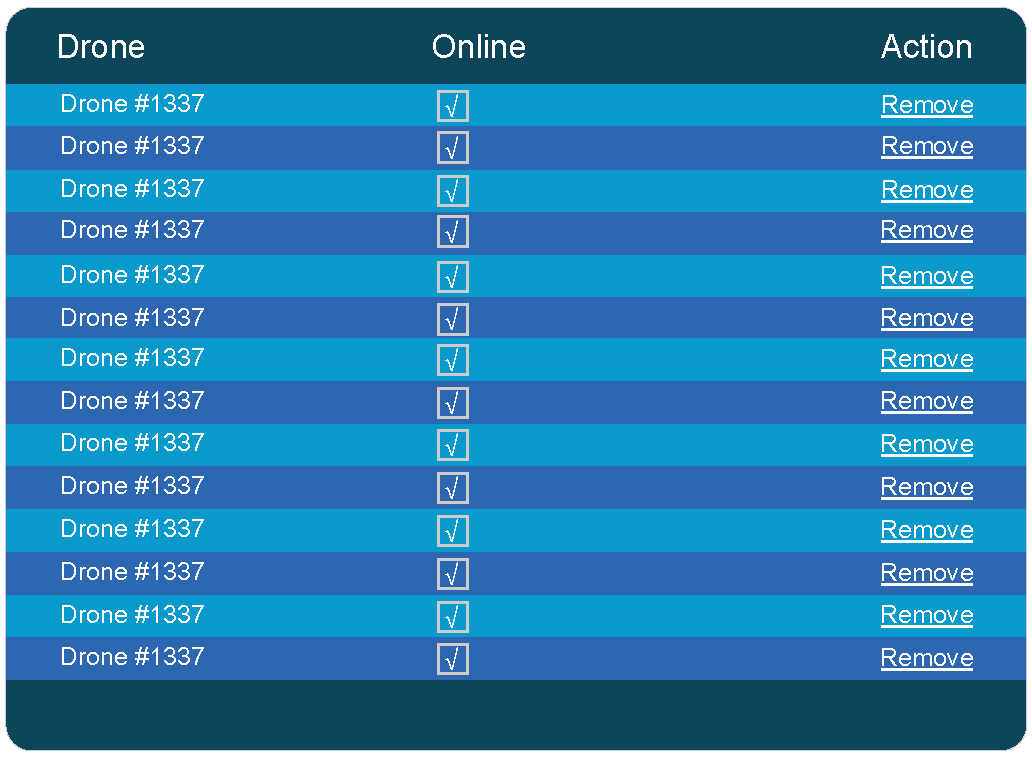
\includegraphics[width=\textwidth]{gfx/table.pdf}
    \caption{Table design for the application}
    \label{fig:table_design}
\end{figure}

\begin{figure}[htb]
    \centering
    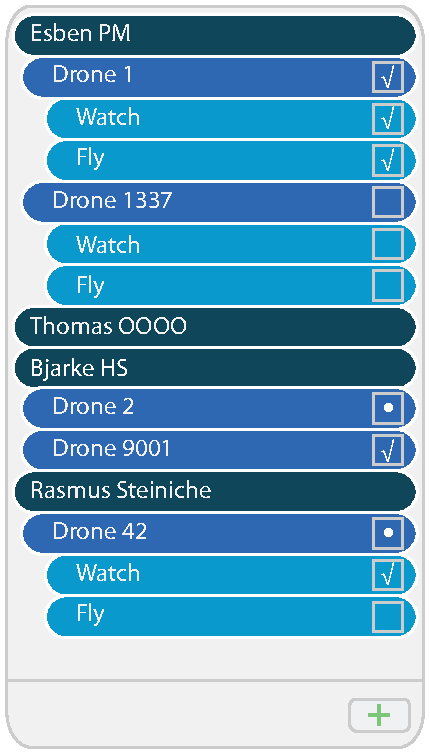
\includegraphics[scale=1.0]{gfx/list.pdf}
    \caption{List design for the application}
    \label{fig:list_design}
\end{figure}

\begin{figure}[htb]
    \centering
    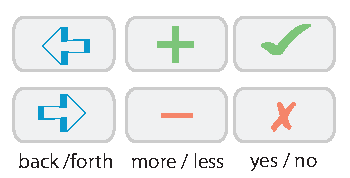
\includegraphics[scale=1.0]{gfx/button.pdf}
    \caption{Button design for the application}
    \label{fig:button_design}
\end{figure}